%\documentclass[runningheads]{llncs}
\documentclass{llncs}

\usepackage{microtype} %This gives MUCH better PDF results!
%\usepackage[active]{srcltx} %DVI search
\usepackage[cmex10]{amsmath}
\usepackage{amssymb}
\usepackage{fnbreak} %warn for split footnotes
\usepackage{url}
\usepackage{qtree} %for drawing trees
%\usepackage{fancybox} % if we need rounded corners
%\usepackage{pict2e} % large circles can be drawn
%\usepackage{courier} %for using courier in texttt{}
%\usepackage{nth} %allows to \nth{4} to make 1st 2nd, etc.
\usepackage{subfigure} %allows to have side-by-side figures
\usepackage{booktabs} %nice tables
\usepackage{multirow} %allow multiple cells with rows in tabular
\usepackage[utf8]{inputenc} % allows to write Faugere correctly
\usepackage[bookmarks=true, citecolor=black, linkcolor=black, colorlinks=true]{hyperref} %For nicer electronic version
\usepackage{fancyvrb} % fancy verbatim package, used with \begin{Verbatim} instead of \begin{verbatim}
\hypersetup{
pdfauthor = {Mate Soos},
pdftitle = {Grain of Salt --- An Automated Way to Test Stream Ciphers through SAT Solvers},
pdfsubject = {TCS'10},
pdfkeywords = {SAT Solver, Stream cipher, Algebraic Cryptanalysis},
pdfcreator = {PdfLaTeX with hyperref package},
pdfproducer = {PdfLaTex}}

%\usepackage{pstricks}
\usepackage{graphicx,epsfig,xcolor}
\usepackage[algoruled, linesnumbered, lined]{algorithm2e} %algorithms

%%%%%%%%%%%%%%%%%%%%%%%%%%%%%%%%%%%%%%%%%%%%%%%%%%%%%%%%%%%
%   to generate the online version of the accepted paper
%%%%%%%%%%%%%%%%%%%%%%%%%%%%%%%%%%%%%%%%%%%%%%%%%%%%%%%%%%%
%\usepackage{butterma} 
%\idline{O.~Kullmann (Eds.): Springer, LNCS 5584}
%\setcounter{page}{244}
%\renewcommand{\year}{2009}
%%%%%%%%%%%%%%%%%%%%%%%%%%

\begin{document}

%%%%%%%%%%%%%%%%%%%%%%%%%%%%%%%%%%%%%%%%%%%%%%%%%%%%%%%%%%%
%   to generate the online version of the accepted paper
%%%%%%%%%%%%%%%%%%%%%%%%%%%%%%%%%%%%%%%%%%%%%%%%%%%%%%%%%%%
%\thispagestyle{electronic}
%%%%%%%%%%%%%%%%%%%%%%%%%%

\title{Grain of Salt --- An Automated Way to Test Stream Ciphers through SAT Solvers}
\author{Mate Soos}
\institute{UPMC LIP6, PLANETE team INRIA, SALSA team INRIA}
%\author{Mate Soos$^\dagger$,
%Karsten Nohl$^\ddagger$, and Claude
%Castelluccia$^\dagger$}
%\institute{$^\dagger$INRIA Rh\^one-Alpes, $^\ddagger$University of Virginia}

\maketitle

\begin{abstract}
In this paper we describe Grain of Salt, a tool developed to automatically test stream ciphers against standard SAT solver-based attacks. The tool takes as input a set of configuration options and the definition of each filter and feedback function of the stream cipher. It outputs a problem in the language of SAT solvers describing the cipher. The tool can automatically generate SAT problem instances for Crypto-1, HiTag2, Grain, Bivium-B and Trivium. In addition, through a simple text-based interface it can be extended to generate problems for any stream cipher that employs shift registers, feedback and filter functions to carry out its work.
\end{abstract}

\section{Introduction}
%%%%%%%%%%
SAT solvers have recently been enjoying a boom in the area of cryptanalysis. It has been shown in multiple papers \cite{DBLP:conf/ima/CourtoisB07,BiviumWithSATsolvers,DBLP:conf/sat/SoosNC09} that SAT solvers are indeed a viable technique in algebraic cryptanalysis to both analyse and potentially break stream or block ciphers. SAT solvers work with problems described in Conjunctive Normal Form (CNF), but obtaining such a problem description is non-trivial. Essentially all works that aimed to analyse a cipher through SAT solvers have developed a way to convert descriptions of ciphers to their CNF form.

In this paper we present Grain of Salt (GoS), a tool that generates optimised CNFs given the description of a stream cipher. It is aimed to be flexible and easy to use, helping the cryptanalyst obtain the best results within the least amount of time. The tool comes loaded with the descriptions of ciphers Crypto-1~\cite{DBLP:conf/esorics/GarciaGMRVSJ08}, HiTag2~\cite{DBLP:conf/isw/CourtoisOQ09}, Trivium~\cite{Canniere06Trivium}, Bivium-B~\cite{Bivium}, and Grain~\cite{DBLP:journals/ijwmc/HellJM07}, but can be easily extended with any stream cipher that uses shift registers, feedback functions and filter functions to carry out its work. The tool is designed to be intuitive to use and general enough to cover a large set of different ciphers while remaining specific enough to address the optimisations possible for the SAT-based cryptanalysis of many stream ciphers.

The rest of this paper is structured as follows. In Sect. \ref{sect:background} we give some background on SAT solvers and SAT-based cryptanalysis. Then, in Sect. \ref{sect:gos-input} we present the input format that GoS uses to describe ciphers. In Sect. \ref{sect:gos-features} we present the various features that GoS offers, and in Sect. \ref{sect:results} we shortly describe the timing results possible with the use of the GoS tool. Finally, in Sect. \ref{sect:conclusions} we conclude this paper.

\section{Background}
\label{sect:background}
In this section we give a short description of SAT solvers and their use in cryptanalysis.%, describe how XOR constraints have been handled and preprocessed in SAT solvers, and describe how Gaussian elimination has been integrated into the DPLL procedure.

\subsection{SAT solvers}
Satisfiability solvers are complex mathematical algorithms used to decide whether a set of constraints have a solution or not. This paper only discusses the well-known conjunctive normal form (CNF) constraint type. The CNF formula $\varphi$ on $n$ binary variables $x_1,\ldots, x_n$, is a conjunction (\texttt{and}-ing) of $m$ clauses $\omega_1,\ldots, \omega_m$ each of which is the disjunction (\texttt{or}-ing) of literals, where a literal is the occurrence of a variable e.g. $x_1$ or its complement, $\neg x_1$.

In this paper we focus on solvers that use the DPLL algorithm. The DPLL procedure is a backtracking, depth-first search algorithm that tries to find a variable assignment that satisfies a system of clauses. The algorithm branches on a variable by assigning it to \texttt{true} or \texttt{false} and examining whether the value of other variables depend on this branching. If they do, the affected variables are assigned to the indicated value and the search continues until no more assignments can be made. During this period, called \emph{propagation}, a clause may become unsatisfiable, as all of its literals have been assigned to \texttt{false}. If such a \emph{conflict} is encountered, a \emph{learnt clause} is generated that captures the wrong variable assignments leading to the conflict. The topmost branching allowed by the learnt clause is reversed and the algorithm starts again. The learnt clauses trim the search tree, reducing the overall time to finish the search. Eventually, either a satisfiable assignment is found or the search tree is exhausted without a solution being found and the problem is determined to be unsatisfiable.

Most DPLL-based SAT solvers understand and deal with problems described in CNF. Usually, a non-trivial part of using SAT solvers is to convert the problem at hand to CNF format. The CNF can then be given to many different SAT solvers, and an appropriate one (e.g. fastest, distributed, etc.) can be selected.

\subsection{SAT Solver-based cryptanalysis}
SAT solver-based algebraic cryptanalysis have successfully been applied to break a number of ciphers secure against other forms of cryptanalysis. The first SAT solver-based algebraic cryptanalysis was by Massacci et al. \cite{Massacci00logicalcryptanalysis}, experimenting with the Data Encryption Standard (DES) using DPLL-based SAT solvers. More recent work by Courtois and Bard has produced attacks against KeeLoq \cite{DBLP:conf/fse/CourtoisBW08} and investigated DES \cite{DBLP:conf/ima/CourtoisB07}. SAT solver-based algebraic cryptanalysis has also been effectively used on modern stream ciphers, such as the reduced version of Trivium, Bivium-B \cite{DBLP:conf/sat/SoosNC09} by Soos et al.

In parallel to the above mentioned papers, there have been multiple tools developed that convert cryptographic functions to CNF. Among them is the python module developed by Martin Albrecht for the \texttt{sage} mathematics platform \cite{SAGE}, \texttt{Logic2CNF} developed by Edd Barrett \cite{Logic2CNF}, and \texttt{STP} (Simple Theorem Prover) by Ganesh et al. \cite{DBLP:conf/cav/GaneshD07}. These tools offer widely different features and can be used at different levels of abstraction. For instance, \texttt{Logic2CNF} only converts a description of the cipher in Algebraic Normal Form (ANF) to CNF, but cannot generate the ANF given a cipher description. \texttt{STP} can parse a complete cipher description but does not retain or deal with the ANF form of the description, thus omitting optimisations possible at that level of abstraction. Finally, the \texttt{sage} module only converts to CNF a description that has already been described in \texttt{sage}, but can use the tools provided by \texttt{sage} to process (and simplify) the problem at the ANF level.

Most of the above mentioned papers and tools implement their own way of describing the cipher in CNF, inventing or re-inventing methods on the way. A well-known reference is the paper by Bard et al. \cite{Bard07efficientmethods} which describes some starting points for the conversion, but individual conversion methods vary widely. Grain of Salt tries to merge the ideas from these papers and tools into one, easy-to-use package.

\section{The input to GoS}
\label{sect:gos-input}
The input to GoS describes a stream cipher in terms of shift registers, feedback, filter and output functions. There are two phases for each attack, the initialisation phase, and the standard running phase. Accordingly, there are two feedback functions associated with each shift register: one that operates during initialisation, and one that operates during normal operation. These feedback functions are often different, as is the case with Crypto-1, Grain and Trivium. Filter functions are always calculated, and their outputs can be used at any point in time by any of the functions, including other filter functions, thus forming a chain. This is important for ciphers such as Crypto-1, where there are multiple micro-filter functions that make up the final output (when in normal mode) and the feedback (when in initialisation mode). The output function is simply a specially designated filter function that produces the output, active only during the normal phase.

Let us now take Grain as an example cipher, and describe it in GoS. Grain has two shift registers, both 80 bits long and its initialisation phase has 160 steps. The main configuration file for this cipher is \texttt{grain/config}, and looks as follows:
\begin{Verbatim}[frame=lines]
sr_size = 80,80                        (1)
linearizable_sr_during_init =          (2)
linearizable_sr_during_norm = 1        (3)
filters = 1                            (4)
init_clock = 160                       (5)
tweakable = sr1-0...63                 (6)
one_out = sr1-64...79                  (7)
\end{Verbatim}

Line \texttt{(1)} tells that there are two shift registers, numbered \texttt{sr0} and \texttt{sr1}. Line \texttt{(2)} means that none of the shift registers' feedback functions are linearizeable during the initialisation phase --- i.e. their feedback functions are non-linear. Line \texttt{(3)} says that during normal operation, shift register \texttt{sr1}'s state is linearizeable, as according to the Grain specification \cite{DBLP:journals/ijwmc/HellJM07}, the second shift register is an LFSR. Line \texttt{(4)} says that the number of filter functions used is one, called \texttt{f0}. The function \texttt{f0} models the complex filter that is used during both the initialisation and the normal phase of the cipher. Line \texttt{(5)} says that the initialisation takes 160 cycles. Line \texttt{(6)} says that the first 64 bits of the second shift register is the IV, i.e. these bits are tweakable (can be freely chosen). Finally, line \texttt{(7)} says that the last 16 bits of the second shift register must be filled with binary ones.

\subsection{Initialisation phase}
The Grain cipher has two phases: the initialisation phase and the normal running phase. Each shift register has to have a feedback function associated with it for each phase. The files describing these functions for Grain must be under the directory \texttt{grain/functions/srX/}, where \texttt{X} is the number of of the shift register (\texttt{0} or \texttt{1} in case of Grain). The feedback of \texttt{sr0} during initialisation is described in the file \texttt{grain/functions/sr0/feedback\_init.txt} shown in Fig. \ref{fig:feedbacks}(a), which corresponds to the line in the Grain specification file
\begin{align*}
b_{i+80} =& s_{i} + b_{i+62} + b_{i+60} + b_{i+52} + b_{i+45} + b_{i+37} + b_{i+33} + b_{i+28} + b_{i+21} +\\
&+b_{i+14} + b_{i+9} + b_{i} + b_{i+63} b_{i+60} + b_{i+37} b_{i+33} + b_{i+15} b_{i+9} +\\
&+b_{i+60} b_{i+52} b_{i+45} + b_{i+33} b_{i+28} b_{i+21} + b_{i+63} b_{i+45} b_{i+28} b_{i+9} +\\
&+b_{i+60} b_{i+52} b_{i+37} b_{i+33} + b_{i+63} b_{i+60} b_{i+21} b_{i+15} +\\
&+b_{i+63} b_{i+60} b_{i+52} b_{i+45} b_{i+37} + b_{i+33} b_{i+28} b_{i+21} b_{i+15} b_{i+9} +\\
&+b_{i+52} b_{i+45} b_{i+37} b_{i+33} b_{i+28} b_{i+21}
\end{align*}
The last line of the file (containing ``\texttt{f0}'') in Fig. \ref{fig:feedbacks}(a) cannot be found in this equation since the filter (modelled with \texttt{f0} in our case) must be XOR-ed into the feedback during the initialisation phase. This filter function is defined in \texttt{grain/functions/f0.txt}, present in Fig. \ref{fig:f0}, which corresponds to the following set of definitions in the Grain specification:
\begin{align*}
z_i =& \sum_{k\in A} b_{i+k} + h(s_{i+3} , s_{i+25} , s_{i+46} , s_{i+64} , b_{i+63})\\
A =& \{1, 2, 4, 10, 31,43, 56\}\\
h(x) =& x_1 +x_4 +x_0 x_3 +x_2 x_3 +x_3 x_4 +x_0 x_1 x_2 +x_0 x_2 x_3 +x_0 x_2 x_4 +x_1 x_2 x_4 +x_2 x_3 x_4
\end{align*}


\newbox\subfigbox
% Create a box to hold the subfigure.
\makeatletter
\newenvironment{subfloat}% % Create the new environment.
{\def\caption##1{\gdef\subcapsave{\relax##1}}%
\let\subcapsave=\@empty % Save the subcaption text.
\let\sf@oldlabel=\label
\def\label##1{\xdef\sublabsave{\noexpand\label{##1}}}%
\let\sublabsave\relax
% Save the label key.
\setbox\subfigbox\hbox
\bgroup}%
% Open the box...
{\egroup
% ... close the box and call \subfigure.
\let\label=\sf@oldlabel
\subfigure[\subcapsave]{\box\subfigbox}}%
\makeatother


\begin{figure}[tb]
\centering
\begin{subfloat}
\begin{minipage}{2.8in}
\small
\begin{Verbatim}[frame=lines]
sr1-0
sr0-62
sr0-60
sr0-52
sr0-45
sr0-37
sr0-33
sr0-28
sr0-21
sr0-14
sr0-9
sr0-0
sr0-63 sr0-60
sr0-37 sr0-33
sr0-15 sr0-9
sr0-60 sr0-52 sr0-45
sr0-33 sr0-28 sr0-21
sr0-63 sr0-45 sr0-28 sr0-9
sr0-60 sr0-52 sr0-37 sr0-33
sr0-63 sr0-60 sr0-21 sr0-15
sr0-63 sr0-60 sr0-52 sr0-45 sr0-37
sr0-33 sr0-28 sr0-21 sr0-15 sr0-9
sr0-52 sr0-45 sr0-37 sr0-33 sr0-28 sr0-21
f0
\end{Verbatim}
\end{minipage}
\caption{Feedback of the NLFSR}
\label{fig:sr0feedback}
\end{subfloat}
\qquad
\begin{subfloat}
\begin{minipage}{1.3in}
\small
\begin{Verbatim}[frame=lines]
sr1-62
sr1-51
sr1-38
sr1-23
sr1-13
sr1-0
f0

















\end{Verbatim}
\end{minipage}
\caption{Feedback of the LFSR}
\label{fig:sr1feedback}
\end{subfloat}
\caption{Feedback functions of Grain used during the initialisation phase. The left-hand figure is stored in the file \texttt{grain/functions/sr0/feedback\_init.txt} while the right-hand figure is stored in the file \texttt{grain/functions/sr1/feedback\_init.txt}}
\label{fig:feedbacks}
\end{figure}

\begin{figure}[tb]
{
\small
\begin{Verbatim}[frame=lines]
sr0-1
sr0-2
sr0-4
sr0-10
sr0-31
sr0-43
sr0-56
sr1-25
sr0-63
sr1-3 sr1-64
sr1-46 sr1-64
sr1-64 sr0-63
sr1-3 sr1-25 sr1-46
sr1-3 sr1-46 sr1-64
sr1-3 sr1-46 sr0-63
sr1-25 sr1-46 sr0-63
sr1-46 sr1-64 sr0-63
\end{Verbatim}
}
\caption{File that describes the filter function for Grain, stored in the file \texttt{grain/functions/f0.txt}}
\label{fig:f0}
\end{figure}

The feedback function of the second filter function during initialisation is present in file \texttt{grain/functions/sr1/feedback\_init.txt}, present in Fig. \ref{fig:feedbacks}(b), which corresponds to the line in the Grain specification
\begin{align*}
s_{i+80} = s_{i+62} + s_{i+51} + s_{i+38} + s_{i+23} + s_{i+13} + s_i
\end{align*}
which again is missing the \texttt{f0}, since the authors of the paper only specified the initialisation phase later, in Sect. 2.1. Here, they make it clear that the filter function, described by \texttt{f0} in our case, needs to be XOR-ed to this feedback function during the initialisation phase.

\subsection{Normal phase}
The feedbacks during normal running look exactly like the feedbacks for initialisation, except for the last lines: the filter function is not XOR-ed in, instead it is simply output as the keystream. Therefore the file describing the feedback of the NLFSR during normal operation, \texttt{grain/functions/sr0/feedback.txt}, is exactly the same as that present in Fig. \ref{fig:feedbacks}(a), with the exception of the last line, \texttt{f0}. Similarly, the file describing the feedback of the LFSR during normal operation is missing the \texttt{f0}. Finally, the file that specifies the keystream, \texttt{grain/functions/output0.txt}, contains just one line with \texttt{f0}, signifying that it is equal to the filter function \texttt{f0}.

\subsection{Composition of filters}
Filter functions, such as \texttt{f0} for Grain can be used extensively in the function descriptions of the cipher. They can also be combined to create some interesting effects. For instance, the output of the Crypto-1 cipher is generated using a set of mini-filter functions as present in Fig. \ref{fig:crypto-1}(b). In the case of Crypto-1, it is best not to describe the final feedback function as one big function, but to preserve the structure of the mini-filter functions. To achieve this, we can define \texttt{f0}\ldots \texttt{f4}, similarly to how we defined filters in Grain, and define the output in \texttt{crypto1/functions/output0.txt}, present in Fig. \ref{fig:crypto-1}(a), as a combination of the internal filter functions.

\begin{figure}[tb]
\centering
\begin{subfloat}
\begin{minipage}{1.7in}
\small
\begin{Verbatim}[frame=lines]
f0
f2 f0
f3 f0
f3 f1 f0
f3 f2 f1
f4
f4 f0
f4 f1 f0
f4 f2 f1 f0
f4 f3
f4 f3 f0
f4 f3 f1
f4 f3 f2 f1
\end{Verbatim}
\end{minipage}
\caption{The output of Crypto-1, described as a function of mini-filter functions \texttt{f0}\ldots \texttt{f4}.}
\label{fig:mini-filters}
\end{subfloat}
\qquad
\begin{subfloat}
\begin{minipage}{2.4in}
\centering
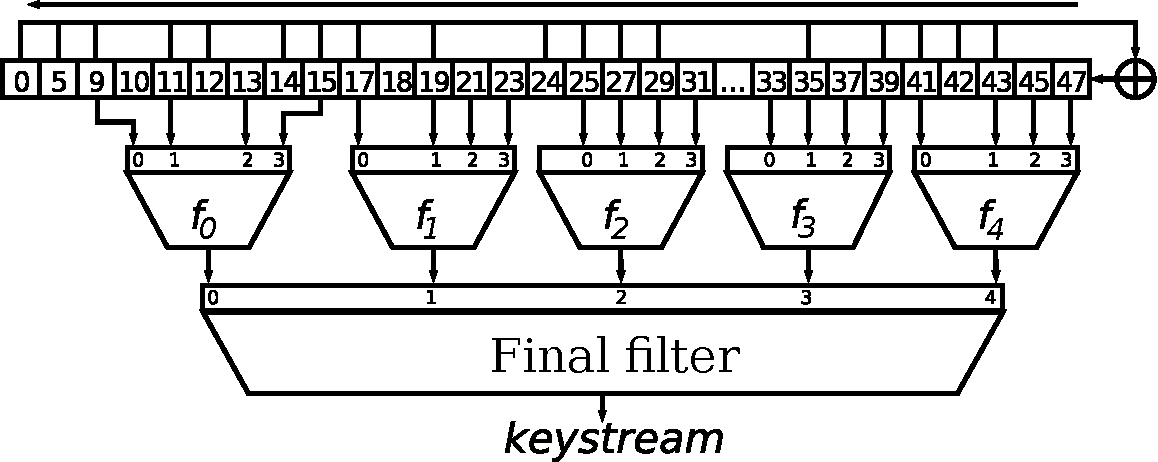
\includegraphics[angle=90, width=2cm]{crypto1_2.pdf}
\end{minipage}
\caption{The functional diagram of the Crypto-1 cipher}
\label{fig:crypto1-diagram}
\end{subfloat}
\caption{The Crypto-1 cipher (on the right), and the description of its final filter function (on the left), made up of multiple micro-functions. The network of micro-functions is clearly visible in the functional diagram, and is replicated in Grain-of-Salt with the use of multiple filter functions.
}
\label{fig:crypto-1}
\end{figure}



\section{Features offered}
\label{sect:gos-features}
The GoS tool offers multiple features to help analyse the stream cipher. We list the most important features here.

\subsection{Variable number of generated output bits}
The number of output bits generated and given to the solver as the base of solving can be chosen at will. The command line switch for this option is \texttt{--outputs NUM}, where \texttt{NUM} is a number that should be sufficient to fully determine the searched-for data. For example, if the initialisation is used for Grain, the number of output bits needed should be at least 80. However, if the initialisation is not used, then at least 160 bits are needed, since the solver has to solve for 160 bits of unknowns (the full state of both shift registers) in that case.

\subsection{ANF generation with fact propagation}
An Algebraic Normal Form of the described cipher with the given number of parameters (described below) can be generated. Various statistical data on the ANF can also be obtained, such as the size (number of monomials) of the each function, the sum size of all functions, etc.

We call fact propagation the effect of evaluating all equations with respect to the given information. The given information can be the output of the cipher or other form of helping information. The evaluations might, for instance, cause a variable to be set instantly, for example, if $a = bc \oplus d$ and $b = \texttt{false}, d=\texttt{true}$ then $a = \texttt{true}$, and by substituting this fact into other equations, further facts could be found. GoS automatically handles this, and recursively propagates all such facts.

Under the aegis of fact propagation GoS also propagates variable equivalences. For example, if $a = bc$ and $c = \texttt{true}$ then $a = b$, which might lead to further facts. For example, the equation $d = b \oplus ab$ would be changed to $d = b \oplus bb = b \oplus b = \texttt{false}$ allowing the propagation of a further fact. Fact and variable equivalence propagation considerably shortens problems, which help when they need to be solved using the SAT solver.

\subsection{CNF Generation}
GoS automatically generates CNF from the fact-propagated ANF using a variety of mechanisms to optimise the conversion. There are mainly two ways of converting an equation in ANF to CNF:
\begin{enumerate}
  \item Through cutting long XOR-s, and introducing internal variables for each monomial of degree $>1$.

  \item Through the use of a Karnaugh map generator~\cite{Karnaugh53Logic}. Karnaugh maps essentially directly generate the CNF from a truth table, needing no conversion. This method was first used in converting cryptographic ANFs by Soos et al. ~\cite{DBLP:conf/sat/SoosNC09}.
\end{enumerate}

Deciding which method to use is non-trivial, and GoS can be given a heuristic cut-off that decides which method to use. The cut-off is given with the command-line parameter \texttt{--karnaugh NUM} where if more than \texttt{NUM} monomials are present in an ANF, the first method is used, while if less or equal, the second method is used to convert to CNF. Essentially, the first method is relatively straight-forward, but can generate very non-optimal representation if the number of monomials is small, their average degree is high and they make use of a small number of variables. For example, the Crypto-1 and HiTag2 ciphers' mini filter functions all fall into this category, and they are best represented as such. However, if for example the degree is low, then the Karnaugh  map representation is uniquely non-optimal, as Karnaugh maps behave the worst (exponentially) for XOR functions, and they also behave very badly with near-XOR functions.

The straight ANF-to-CNF method of simply converting the XOR to CNF and then introducing internal variables for monomials of degree $>$ 1 is done as follows. Long XOR-s must be cut due to the exponential nature of their conversion: an $n$-long XOR can only be represented (without introduction of internal variables) as $2^{n-1}$ clauses. To overcome this, XOR-s are cut such as:
\begin{align*}
a \oplus b \oplus c \oplus d \oplus e \oplus f =& \texttt{true}
\leftrightarrow\\
a \oplus b \oplus c \oplus i =& \texttt{false}\\
d \oplus e \oplus f \oplus i =& \texttt{true}\\
\end{align*}
but the best limit at which XOR-s must be cut, which is usually called the \emph{cutting number} is not easy to determine. The default is 7 in GoS, but can be changed with \texttt{--xorcut NUM}. Monomials are expressed in the CNF language through the introduction of internal variables. For example, the monomial $ab$ is expressed as $i_2 = ab$, leading to the clause-set:
\begin{align*}
\neg i_2 \vee b\\
\neg i_2 \vee a\\
i_2 \vee \neg a \vee \neg b\\
\end{align*}

An optimisation for the straight ANF-to-CNF conversion is that monomials in the CNF world can contain negations, i.e. it is no longer necessary to write $a \oplus ab$, since that can be simply written as $a(1+b)=a\neg b$. This optimisation can be applied recursively. For example:
\begin{align*}
a \oplus b \oplus ab \oplus c \oplus cd =& \texttt{true}
\leftrightarrow&\\
b \oplus a(1\oplus b) \oplus c(1\oplus d) =& \texttt{true}
\leftrightarrow&\\
1 \oplus (1\oplus a)(1\oplus b) \oplus c(1\oplus d) =& \texttt{true}
\leftrightarrow&\\
\neg a\neg b \oplus c\neg d =& \texttt{false}
\end{align*}
reducing the original 5 monomials into a mere two. Representing these monomials that are not free of negations takes exactly the same amount of resources in CNF as representing those that are free of negations, leading to a potential overall reduction in the final CNF. The reduction is only potential, as the internal variables that represent monomials that are used in multiple places need only be described once, and the extended monomials could possibly make it more difficult for the same monomials to appear, limiting their benefits. Therefore, this optimisation can be turned off with the command-line switch \texttt{--noextmonomials}. The default is for this optimisation to be turned on, as we have experienced speedups using it.

\subsection{Dependency tree generation}
It is assumed that only the output of the stream cipher is known to the attacker. Therefore, functions that are not connected in some way to the output of the function can be discarded: they are internal variables that need not be calculated, since they cannot help solving the internal state. To remove these functions, a dependency tree is generated that takes as root all the output bits of the cipher, and generates a tree that reaches the original internal state bits. All functions that are not connected to this tree can be discarded.

Dependency tree generation is very important, as it lets the designer describe as many filter functions as he or she wishes: the functions that are not used will not hamper the solving. For example, some ciphers use filter functions that are specific to the initialisation phase. Without dependency tree generation, these filter functions would be calculated (but not used) during the normal running phase, slowing down the solver.

\subsection{Solving with and without initialisation phase}
The GoS tool has two running modes. It can either try to solve for the non-tweakable and non-oned-out parts of the cipher when initialisation is turned on, or it can solve for the entire state when initialisation is turned off. In other words, the two typical scenarios are covered: either the IV is known, the key is unknown, and the initialisation is carried out, or the entire state of the cipher is unknown, but the initialisation is not carried out. This behaviour can be simply switched using a command line switch \texttt{--init yes} or \texttt{--init no}.

Typically, with the initialisation turned on, the number of bits to be solved is much less. For example, in the case of Grain, the IV is 64, and the one-ed out part is 16 bits, so only 80 bits of the first shift register (i.e. the key) is the unknown. However, the initialisation takes 160 cycles, which greatly increases the difficulty of the resulting set of equations. On the other hand, without initialisation, the number of unknown bits increases to 2*80 = 160, but since initialisation is not carried out, most equations are very short.

\subsection{Base shifting}
Base shifting can be activated when solving without initialisation. Base shifting is the name we use for the technique first presented in \cite[Sect. 4.3]{DBLP:conf/sat/SoosNC09}. There, the authors show that the base unknown of the cipher can be \emph{any} moment in time. So, for example, if the number of output bits generated is 200, and no initialisation is used, then the cipher is clocked for 100 bits, with a total length of 100 + 80 = 180 (since 80 is the original size of each). Any consecutive 80 bit frame of this can be taken as the unknown, as the feedback functions can be re-arranged to clock backwards for these ciphers. This is very advantageous, as typically, the complexity increases exponentially starting from a point $T$, and if we take $T$ to be near the middle of the time-frame (e.g. at $T=90$ in our example), then the total complexity of the generated functions are much less than if we had taken the typical approach, i.e. to take $T=0$.

%TODO add example graphs

The command line parameter for base shifting is \texttt{--base-shift NUM} where \texttt{NUM} must be smaller or equal to the number of output bits. For this to work with $\texttt{NUM}>0$, the feedback functions of the cipher must be reversible. This is true for Crypto-1, HiTag2, Bivium-B, Trivium, and Grain. Stream ciphers can be created where this is not the case --- these stream cipher are, however, usually constrained in that it is hard to make them work faster through parallel implementation of the feedback and filter functions in hardware.%, since reversing exploits exactly the same mechanism.

As a concrete example, let us take the Grain cipher, without the initialisation phase switched off. If the number of output bits generated is 200, the base shifting can be any number between 0 and 200. For a shifting number $x$, the unknowns are the states of the shift registers at time $x$. In other words, if we take each shift register as a memory line that does not forget its old contents, then the unknowns are the state variables $x\ldots x+80$ of both shift registers. We call these variables the \emph{reference state variables}. When initialisation is turned on, the reference state variables are simply the variables that are neither tweakable nor one-ed out, i.e. they are the state variables where (typically) the key is loaded.

\subsection{Help bit calculation}
Help bits are data pieces that are given such that it is easier to solve for the state of a cipher. These are important, as it is infeasible to wait immense amounts of time to check whether, for example, the state of Grain can be solved. In order to circumvent this problem, we give some reference state variables as \emph{help bits} to the solver, such that it can solve faster.  Once the solving has finished, one can estimate the time it would take to solve for the whole state of the cipher, without the help bits. The GoS tool offers two types of help bit calculations. One is a probabilistic calculator, and the other is a deterministic calculator, and both employ a Monte-Carlo method to achieve their goals. For the following sections, let us assume that $V$ the possible set of variables that can be help bits (i.e. $V$ contains exactly the reference state variables).

The Monte-Carlo method, first introduced by Metropolis and Ulam~\cite{Monte-Carlo-method} is used in many areas of research such as integration and computer security (e.g. the Rabin primality test~\cite{Rabin-primality-test}). It is essentially a randomised algorithm that samples a tiny part of the possibly immense space and processes the results to approximate an unknown value for the whole space. In case of the Rabin primality test, the Monte-Carlo algorithm uses a randomised test to decide if a positive integer is a prime or not. The algorithm has a certain chance ($<1/4$) to give a false negative result, but running the algorithm many times essentially eliminates the chance that a number is composite.

\subsubsection{Deterministic method}
Since using different reference state variables as help bits could give different timings, it is non-trivial which ones to use. To achieve maximum performance, we use an approach that we have found to be adequate to find a good set.

We first generate the ANF that describes the cipher given all settings. Then, we set a variable $v \in V$, $v \leftarrow \texttt{true}$, and \emph{propagate} all changes. We count the number of monomials in the resulting ANF. Then, we set $v\leftarrow \texttt{false}$, and again count the size of the resulting ANF. The sum of these two values is the ``score'' for this help bit. We perform these steps for each variable in $L$, and the one that has the smallest score wins. We now put this winning variable into the ordered set $H$, and continue the search as follows.

Let us call $L$ the possible set of variables that can be help bits (i.e. $L$ contains exactly the reference state variables). We take a variable $v \in L\backslash H$ and randomly set all variables in $H$, plus we set $v \leftarrow \texttt{true}$, and count the score. We do ten such measures, each time setting the variables in $H$ randomly, and sum the scores. Then, we do the same, but with  $v \leftarrow \texttt{false}$, and sum the scores. The sum of these 20 measurements will be the score for this $v$. We do this for all $v \in L \backslash H$: the variable with the smallest score wins and enters $H$. At the end of the algorithm, we reach a point where $L\backslash  H = \emptyset$, and all variables have been ordered in $H$.

The presented algorithm is a randomised greedy algorithm that tries to find a local minima at each point. Since even a local minima is very difficult to find, the algorithm probabilistically tries to find this local minima, through 20 random tests. For better local minima finding, the number 20 can be increased to any even number, ameliorating the algorithm.

We have found this algorithm to be very powerful in reducing the time to solve a given cipher. Without such ordering of bits, the speed to solve a certain problem can be hundreds of times more difficult. The output of this algorithm is simply put a file called ``best-bits'', and the variable numbers are simply listed one after the other. If the cryptographer knows a better ordering, this file can simply be overwritten.

Once the ``best bits'' file has been generated, it can be used from the program by giving the option \texttt{--deterBits NUM}, where \texttt{NUM} is the number of best bits the program should set randomly when generating the problem instances. Averaging the time it takes to solve these problems and multiplying the average by $2^{\texttt{NUM}}$ one gets the amount of expected time to solve the cipher.

The program specifically does not include a method to break a cipher, though given a specific cipher output, it could generate all $2^{\texttt{NUM}}$ possible problems. Naturally, one of the generated problems would actually break the given output stream, revealing the key or the state of the cipher (depending on whether initialisation was enabled or not).

\subsubsection{Probabilistic method}
The probabilistic method is activated with the command line switch \texttt{--probBits NUM} and it simply randomly sets a random set of \texttt{NUM} variables from $L$ and does many runs of these random configurations. The time it takes to solve these randomly picked instances is then averaged. %These randomisation steps have helped us to effectively generate high-quality random instances, and thus evaluate with high confidence the time it takes to break a cipher given a certain number of variables. 

To approximate the time it takes to attack the cipher without giving any variables we use the following technique. We run many instances of the above algorithm with $\texttt{NUM}=n, n-1, \ldots n-k$ number of reference state variables, where $n$ is small enough such that the algorithm is not trivial to solve, and $n-k$ is as small as possible such that the resulting system is still solved within a reasonable amount of time. The average time is then plotted against the number of reference state variables given, and the plot is extrapolated to the point where there are no reference state variables given.

Although there is no proof that at any point during $\texttt{NUM}=n-k-1\ldots 0$ the graph does not suddenly change, we believe this to be extremely unlikely. For the explication of the reasons, let us first define some notions. Let us define two problems for a given cipher: problem $A$ is when $\texttt{NUM}=x$, and problem $B$ is where $\texttt{NUM}=x-1$, where $n \geq x>0$ but otherwise $x$ is irrelevant. Let us assume, without loss of generality, that $V'$ is the set of reference variables selected to be assigned in $B$. Let the set of reference variables assigned in $A$ be $V' \bigcup v$. We can now list the reasons why we believe the graph does not deviate from a straight line if the time is plotted in a logarithmic scale:
%
\begin{itemize}
 \item Every problem in $B$ can be directly mapped to $2|V\setminus V'|=2(n-x+1)$ problems in $A$. Since the underlying algorithm of DPLL-based SAT solvers is essentially an intelligent brute-force, we can safely assume it does not behave worse than a brute-force, and solves the problem $B$ in at most twice the time than solving any problem in $A$. This is further underlined by our observation that SAT solvers branch on the reference state variables --- thus the first branching of the solver when solving $B$ will indeed be a variable from $|V\setminus V'|$
 
 \item The more choice of variables a SAT solver has to branch on, the better the dynamic variable branch ordering will work. This means that it is expected of the solver to solve in less than twice the time problem $B$ with a choice of $n-x$ branch variables, than two problems in $A$ with a choice of $n-x-1$ branch variables
 
 \item Clauses learnt during the solving of $A$ that are independent of the setting of variable $v$ cannot be reused between the solving instances. Therefore, it is expected that problem $B$ can be solved faster than two problems in $A$, as the solver in the former case does not need to re-learn these same clauses
 
 \item The underlying problem structure does not change between problem $A$ and problem $B$
 
 \item It is the same underlying randomised solving algorithm that is used to solve both problem $A$ and problem $B$
\end{itemize}

The extrapolation is usually straightforward if a large enough number of randomisation steps are involved: the plotted graph is straight if plotted against a logarithmic time. We note that the possibility of extrapolation is an advancement over previous attempts. Previous attempts failed, as they did not introduce sufficient randomness into the system. This lack of suitable randomisation meant that their results were not extrapolateable~\cite{BiviumWithMiniSat,BiviumWithSATsolvers}.

\section{Results}
\label{sect:results}
GoS in conjunction with an appropriate SAT solver such as CryptoMiniSat~\cite{CryptoMiniSat} can be used to break Crypto-1 in 40~s, HiTag2 in $2^{14.5}$~s, and Bivium-B in an approximated $2^{36.5}$~s using a a Xeon E5345@2.33GHz computer. All these figures are faster than exhaustive search, leading to the breaking of these algorihtms. In the literature we have not found any results that indicated a faster solving time for these ciphers using a SAT-based cryptanalsysis, and so we believe these figures to be the current state-of-the-art.

\section{Conclusions}
\label{sect:conclusions}
%%%%%%%
We have presented Grain of Salt, an integrated package to test stream ciphers against SAT solver-based attacks. The tool can flexibly generate with a minimum of user intervention a CNF representation of any shift-register based stream cipher, helping the researcher evaluate the cipher against SAT solver-based algebraic attacks. The input language and the command line options of the tool are easy to use and user-friendly, helping the novice as well as the advanced users to profit from the tool. We envision that Grain of Salt will be further extended by researchers to carter for their specific needs, making the tool more diverse and more useful for the whole of the research community.

\section*{Acknowledgements}
The author was supported by the RFID-AP ANR Project, project number \texttt{ANR-07-SESU-009}. I would like to thank Karsten Nohl for some initial ideas, notably base-shifting.

\bibliographystyle{splncs}
\bibliography{sigproc}

\vfill
\pagebreak

\end{document}
